%!TEX root =机械设计.tex
\chapter{链传动}
在学完这一章之后最大的收获其实是知道了自行车为啥会响（

和上一节的带传动相比，由于链传动是链轮轮齿和链节啮合传动，所以链传动的{\color{red}\text{平均传动比}}准确，传动效率高，压轴力小，能在温度较高、有油污的恶劣环境条件下工作。对，适合用在自行车上。

但缺点也很明显啊。瞬时传动比不恒定，传动平稳性差，工作中有冲击和噪声,不宜在急速变载和变向的传动中使用。

\section{传动链的结构}
传动链主要分为滚子链和齿形链。课程掌握滚子链为主。
\subsection{滚子链结构}
滚子链的结构如下图：
\begin{figure}[htbp]
    \centering
    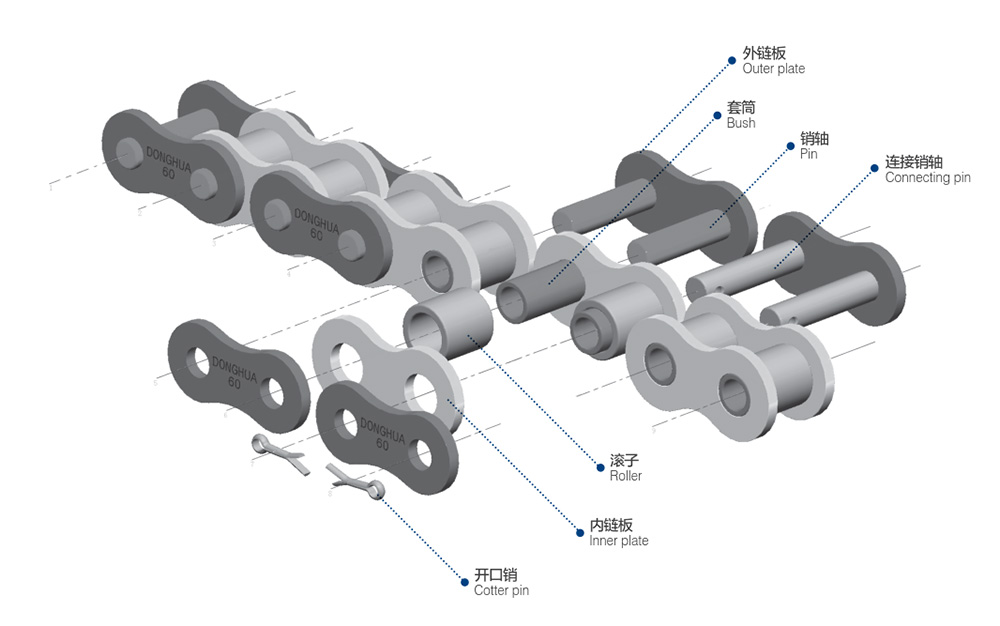
\includegraphics[width=0.9\textwidth]{Figure/滚子链结构.jpg}
    \caption{滚子链结构}
    \label{fig:滚子链结构}
\end{figure}

观察这个滚子链的结构，可以看出以下特点:
\begin{itemize}
    \item 链板制成“8”字形，目的是使各截面抗拉强度近似相等并减少质量及惯性力
    \item 内外链板间有间隙，保证润滑油能进入磨损面（主要磨损面是套筒和销轴之间）
\end{itemize}

然后滚子链各部件之间的配合关系如下：
\begin{itemize}
    \item 内链板和套筒之间采用过盈配合
    \item 外链板和销轴之间采用过盈配合
    \item 套筒和销轴之间采用间隙配合
    \item 滚子和套筒之间采用间隙配合
\end{itemize}

\begin{proposition}
    滚子链的接头型式
\end{proposition}
